
\section{Auswertung}
\label{sec:Auswertung}
\subsection{Verifikation der Linsengleichung}
Die Ergebnisse der ersten Messung sind in Tabelle \ref{tab:M1} aufgetragen.
\begin{figure}[hp]
	\begin{minipage}{0.49\textwidth}
		\centering
		\begin{tabular}{S[table-format=3] S[table-format=3] S[table-format=3.2]}
			\toprule
			\multicolumn{3}{c}{Linse mit $\tilde{f}=\SI{100}{\milli\meter}$}\\
			%\multicolumn{3}{c}{f_1=100\,\si{\milli\meter}} & \multicolumn{3}{c}{f_2=50\,\si{\milli\meter}} \\
			{$g_1/\:\si{\milli{\meter}}$} & {$b_1/\:\si{\milli{\meter}}$} & {$f_1/\:\si{\milli{\meter}}$} \\	
			\midrule
			120 & 525 & 98.09\\
			130 & 390 & 98.64\\
			140 & 319 & 97.59\\
			150 & 277 & 96.96\\
			160 & 251 & 95.63\\
			170 & 227 & 97.20\\
			180 & 204 & 97.71\\
			190 & 198 & 97.31\\
			200 & 192 & 97.30\\
			210 & 186 & 97.50\\
			220 & 177 & 97.67\\
			\bottomrule
			\end{tabular}
	\end{minipage}
	\begin{minipage}{0.49\textwidth}
		%\centering
		\begin{tabular}{S[table-format=3] S[table-format=3] S[table-format=3.2]}
			\toprule
			\multicolumn{3}{c}{Linse mit $\tilde{f}=\SI{50}{\milli\meter}$}\\
			%\multicolumn{3}{c}{f_1=100\,\si{\milli\meter}} & \multicolumn{3}{c}{f_2=50\,\si{\milli\meter}} \\
			{$g_2/\:\si{\milli{\meter}}$} & {$b_2/\:\si{\milli{\meter}}$} & {$f_2/\:\si{\milli{\meter}}$}\\	
			\midrule
				60  & 2700 & 124.14 \\
				70  & 1570 & 117.98 \\
				80  & 1210 & 111.22 \\
				90  & 1040 & 104.35 \\
				100 &  920 &  97.65 \\
				110 &  870 &  90.20 \\
				120 &  800 &  82.83 \\
				130 &  770 &  75.04 \\
				140 &  750 &  67.01 \\
				150 &  720 &  58.70 \\
			\bottomrule
			\end{tabular}
		\end{minipage}
	\caption{Messung der Bildweiten $b_i$ bei festgelegter Gegenstandsweite $g_i$ sowie die daraus berechneten Brennweiten nach der Linsengleichung.}
	\label{tab:M1}
\end{figure}
Für die berechnete Brennweite ergeben sich Werte von 
\begin{align}
	f_1 &= \SI{0.104(6)}{\meter}\\
	f_2 &= \SI{0.087(11)}{\meter}.
\end{align}
Das $b$-$g$-Diagramm \ref{fig:bgdiagramm} zeigt dadurch, dass sich die Linien auf einem nicht-punktförmigen Gebiet untereinander schneiden, die Unsicherheit der Messergebnisse an.
Die Mittelwerte weichen von der Herstellerangabe, $\tilde{f_1}=\SI{0.1}{\meter}$ und $\tilde{f_2}=\SI{0.05}{\meter}$, um 
\begin{align}
	\mathup{\Delta}f_1 &= 4\% \\	
	\mathup{\Delta}f_2 &= 42.5\%
\end{align}
ab.
Daher ist für die Linse $f_1$  die Brennweite $f$ über die Linsengleichung \eqref{eq:linsengleichung} verifizierbar, für die Linse $f_2$ weicht die berechnete Brennweite stark ab.

\begin{figure}[hb] %% b-g-Diagramm
	\centering
	\begin{subfigure}{0.9\textwidth}
	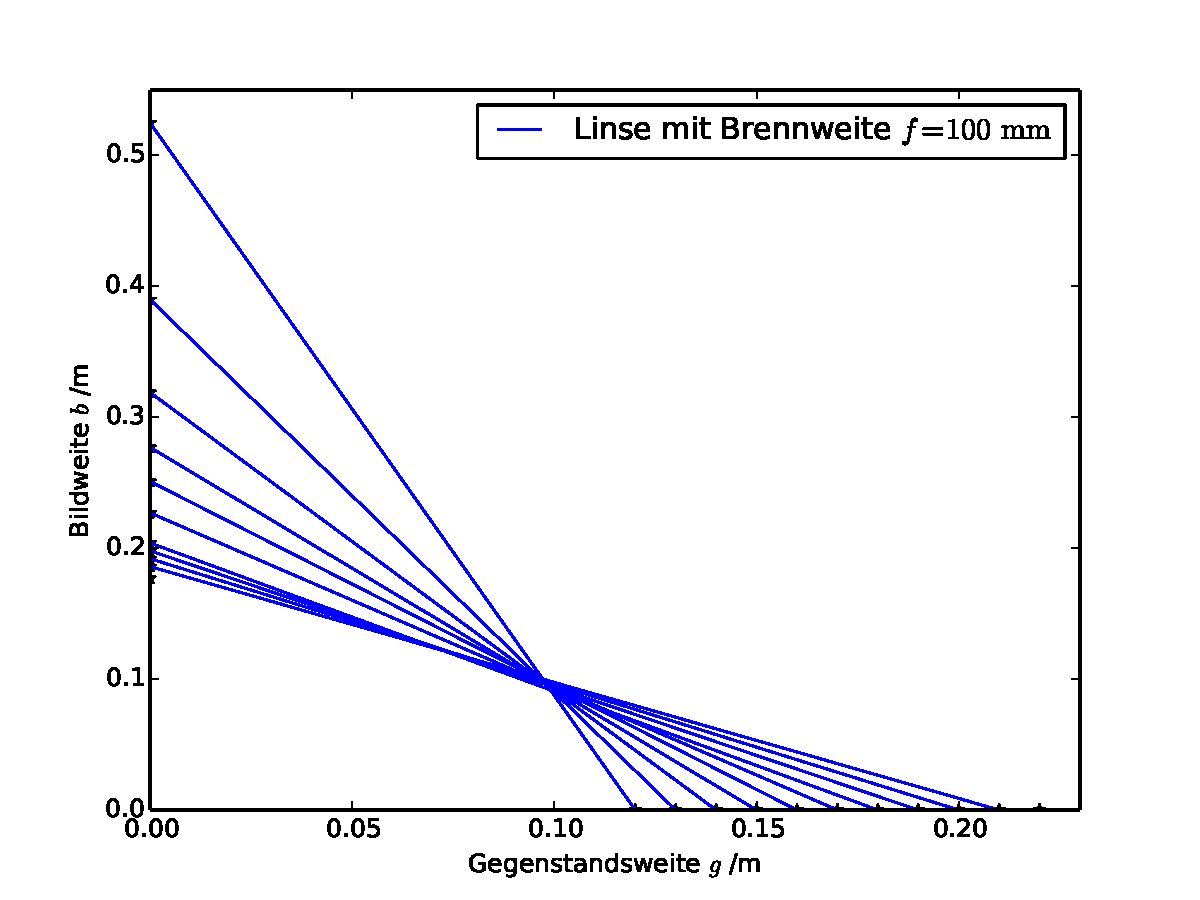
\includegraphics[width=\textwidth]{Bilder/Messung1.pdf}
	\end{subfigure}
	\begin{subfigure}{0.9\textwidth}
	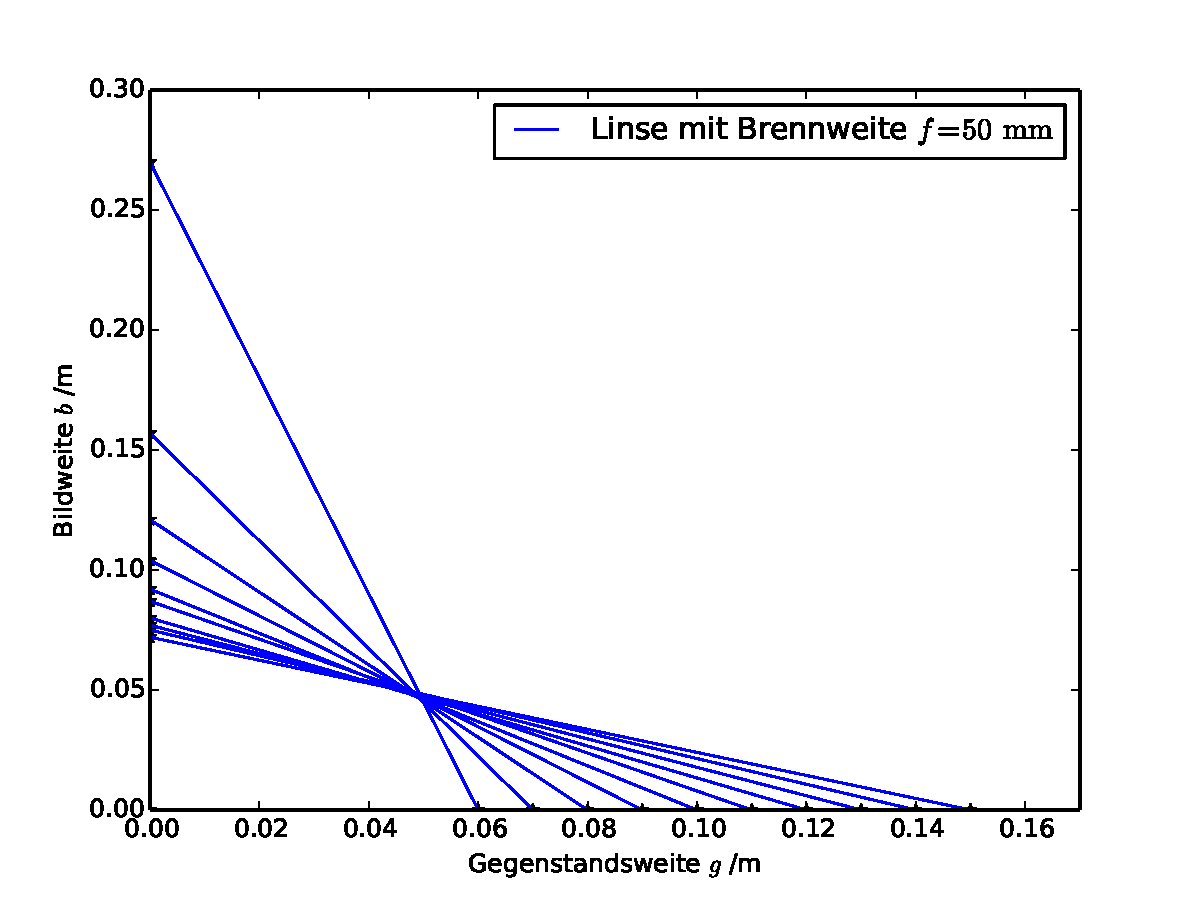
\includegraphics[width=\textwidth]{Bilder/Messung2.pdf}
	\end{subfigure}
	\caption{$b$-$g$-Diagramme zur Darstellung der Messgenauigkeit.}
	\label{fig:bgdiagramm} 
\end{figure}


\subsection{Methode nach Bessel}
Die Ergebnisse der Messung nach dem Bessel-Verfahren sind in Tabelle \ref{tab:M2} aufgetragen.
\begin{table}[htp]
	\centering
	\begin{tabular}{S[table-format=3.0] S[table-format=2.1] S[table-format=2.1] S[table-format=3.2] S[table-format=2.1] S[table-format=2.1] S[table-format=3.2]}
	\toprule
	&\multicolumn{3}{c}{Linsenposition 1} & \multicolumn{3}{c}{Linsenposition 2} \\
		{$e/\:\si{\milli{\meter}}$} & {$g_1/\:\si{\milli{\meter}}$} & {$b_1/\:\si{\milli{\meter}}$} & {$f_1/\:\si{\milli{\meter}}$} & {$g_2/\:\si{\milli{\meter}}$}  & {$b_2/\:\si{\milli{\meter}}$} & {$f_2/\:\si{\milli{\meter}}$}\\	
		\midrule
		450 & 14.4 & 30.6 & 112.36 & 14.2 & 30.8 & 112.35 \\
		500 & 13.4 & 36.6 & 124.73 & 13.5 & 36.5 & 124.74 \\
		550 & 12.7 & 42.3 & 137.10 & 12.7 & 42.3 & 137.10 \\
		600 & 12.2 & 47.8 & 149.47 & 12.3 & 47.7 & 149.48 \\
		650 & 11.9 & 53.1 & 161.85 & 12.0 & 53.0 & 161.85 \\
		700 & 11.8 & 48.2 & 174.53 & 11.7 & 58.3 & 174.24 \\
		750 & 11.6 & 73.4 & 186.23 & 11.5 & 73.5 & 186.22 \\
		800 & 11.4 & 68.8 & 198.98 & 11.6 & 68.8 & 198.99 \\
		850 & 11.4 & 73.6 & 211.36 & 11.4 & 73.6 & 211.36 \\
		900 & 11.3 & 78.7 & 223.74 & 11.3 & 78.8 & 223.73 \\
			\bottomrule
		\end{tabular}
	\caption{Messung der Bild- und Gegenstandsweiten $b_i$ und $g_i$ bei festgelegtem Abstand $e$ nach Bessel; weißes Licht.}
	\label{tab:M2}  %% Weißes Licht, Bessel
\end{table}
Für die berechnete Brennweite ergibt sich ein Wert von 
\begin{equation}
	f = \SI{0.168(12)}{\meter}
\end{equation}
Der berechnete Mittelwert weicht von der Herstellerangabe $\tilde{f}=\SI{0.1}{\meter}$ um 68\% ab.

Die Ergebnisse der Messung mit einfarbigem Licht sind in den Tabellen \ref{tab:M2a} und \ref{tab:M2b} aufgetragen.
Die ermittelten Brennweiten betragens
\begin{align}
	f_\text{Rot} &= \SI{0.1141(7)}{\meter}\\
	f_\text{Blau} &= \SI{0.073(16)}{\meter}
\end{align}
und zeigen damit die Abhängigkeit der Brechung von der Wellenlänge des Lichtes.
\begin{table}[p]
		\centering
		\begin{tabular}{S[table-format=2.0] S[table-format=3.0] S[table-format=3.0] S[table-format=3.2] S[table-format=3.0] S[table-format=3.0] S[table-format=3.2] }
		\toprule
			&\multicolumn{3}{c}{Linsenposition 1} & \multicolumn{3}{c}{Linsenposition 2} \\
			{$e/\:\si{\milli{\meter}}$} & {$g_{1,\mathup{r}}/\:\si{\milli{\meter}}$} & {$b_{1,\mathup{r}}/\:\si{\milli{\meter}}$} & {$f_{1,\mathup{r}}/\:\si{\milli{\meter}}$} & {$g_{2,\mathup{r}}/\:\si{\milli{\meter}}$} & {$b_{2,\mathup{r}}/\:\si{\milli{\meter}}$} & {$f_{2,\mathup{r}}/\:\si{\milli{\meter}}$} \\	
			\midrule
			50 & 143 & 307 & 111.88 & 306 & 144 & 111.89  \\
			60 & 126 & 424 & 113.00 & 424 & 126 & 113.00 \\
			70 & 118 & 532 & 114.38 & 531 & 119 & 114.38 \\
			80 & 117 & 633 & 115.82 & 636 & 117 & 115.82 \\
			90 & 115 & 735 & 115.45 & 739 & 111 & 115.45 \\
			\bottomrule
			\end{tabular}
			\caption{Messung der Bild- und Gegenstandsweiten $b_i$ und $g_i$ bei festgelegtem Abstand $e$ nach Bessel; rotes Licht.}
			\label{tab:M2a} %% Farbiges Licht, Bessel
\end{table}
\begin{table}[p]
			\centering
			\begin{tabular}{S[table-format=2.0] S[table-format=3.0] S[table-format=3.0] S[table-format=3.2] S[table-format=3.0] S[table-format=3.0] S[table-format=3.2] }
			\toprule	
				&\multicolumn{3}{c}{Linsenposition 1} & \multicolumn{3}{c}{Linsenposition 2} \\
				{$e/\:\si{\milli{\meter}}$} & {$g_{1,\mathup{b}}/\:\si{\milli{\meter}}$} & {$b_{1,\mathup{b}}/\:\si{\milli{\meter}}$} & {$f_{1,\mathup{b}}/\:\si{\milli{\meter}}$} &{$g_{2,\mathup{b}}/\:\si{\milli{\meter}}$}  & {$b_{2,\mathup{b}}/\:\si{\milli{\meter}}$} & {$f_{2,\mathup{b}}/\:\si{\milli{\meter}}$}\\	
				\midrule
				50 & 366 & 134 & 97.15 & 132 & 368 & 97.15 \\
				60 & 477 & 123 & 97.19 & 122 & 478 & 97.19\\
				70 & 782 & 118 & 15.63 & 116 & 784 & 15.63\\
				80 & 784 & 116 & 58.88 & 114 & 786 & 58.89\\
				90 & 788 & 112 & 97.31 & 111 & 789 & 97.31\\
				\bottomrule
			\end{tabular}
			\caption{Messung der Bild- und Gegenstandsweiten $b_i$ und $g_i$ bei festgelegtem Abstand $e$ nach Bessel; blaues Licht.}
			\label{tab:M2b}
\end{table}

\subsection{Methode nach Abbe}
\begin{table}[ht]
	\centering
	\begin{tabular}{S[table-format=3.0] S[table-format=3.0] S[table-format=2.0] S[table-format=1.2]}
	\toprule
		 {$g'/\:\si{\milli{\meter}}$} & {$b'/\:\si{\milli{\meter}}$} & {$B/\:\si{\milli{\meter}}$} & {$V/\:\si{\milli{\meter}}$}\\	
		\midrule
		200 & 790 & 80 & 2.67\\
		250 & 551 & 44 & 1.47\\
		300 & 480 & 31 & 1.03\\
		350 & 416 & 25 & 0.83\\
		400 & 398 & 20 & 0.67\\
		450 & 380 & 17 & 0.57\\
		500 & 370 & 15 & 0.50\\
		550 & 346 & 13 & 0.43\\
		600 & 348 & 11 & 0.37\\
		650 & 336 & 11 & 0.37\\
	\bottomrule
	\end{tabular}
	\caption{Messwerte zur Bestimmung der Brennweite des Linsensystems nach Abbe.} %% Abbe
\end{table}
